\chapter{Construction}
\label{chapter:construction}
\section{PREESM Filter Application}
An actor network is constructed in PREESM that represents the video filter
application. The final PiSDF model of the PREESM video filter application is
presented in figure \ref{preesm_actors}. The PREESM filter application is
adapted from the PREESM tutorial at \cite{preesmtut} by adding another
processing path for gaussian filter and making the necessary modifications to
the shared parts of the application.

\begin{figure}[h!] \label{preesm_actors} \begin{center}
    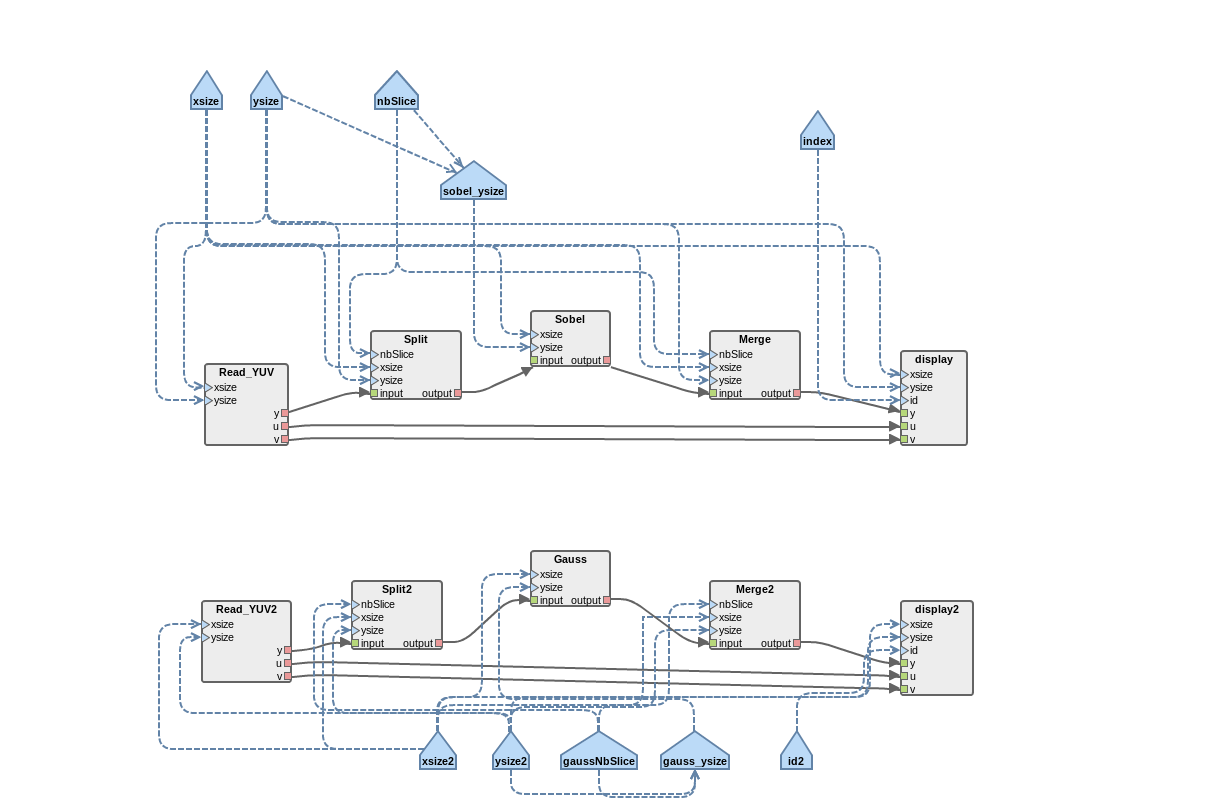
\includegraphics[width=0.99\textwidth]{images/preesm_diagram.png}
    \caption{The PiSDF graph of the PREESM filter application} \end{center}
\end{figure}

To keep the model simple and the program well analyzable both of the processing
paths in the network are independent.

The first actor on both of the processing paths loads the video frames from
memory and passes them to splitting actors. The splitting actor splits the
frames to a suitable number of splices to enable processing of the same video
stream on multiple cores. The filter actor follows the splitting actor. Partial
frames filtered in the filter actor are merged back to whole frames in the merge
actors. The last actors on both of the processing paths are dummy actors.\\

TODO: explain scheduling

\section{OpenEM Filter Application}
\section{PSE Model of OpenEM Filter Application}
\section{Instrumentation}
